\subsection{Среда CartPole}

CartPole — это классическая задача теории управления, описанная в \cite{cartpole}. Она представляет собой тележку, которая может двигаться по одномерному треку без трения. К каретке с помощью шарнира прикреплен неустойчивый шест, центр тяжести которого находится выше точки опоры. Задача когнитивного агента заключается в том, чтобы не дать шесту упасть, прикладывая импульсы силы к каретке. 

С точки зрения когнитивного моделирования, сложность задачи состоит в том, что агент изначально не знает законов физики (гравитации, инерции, массы объектов). Он должен самостоятельно сформировать внутреннее представление динамики системы исключительно на основе поступающих числовых сигналов.

\begin{figure}[h!] % [h!] - попытка разместить картинку "здесь" (here)
    \centering
    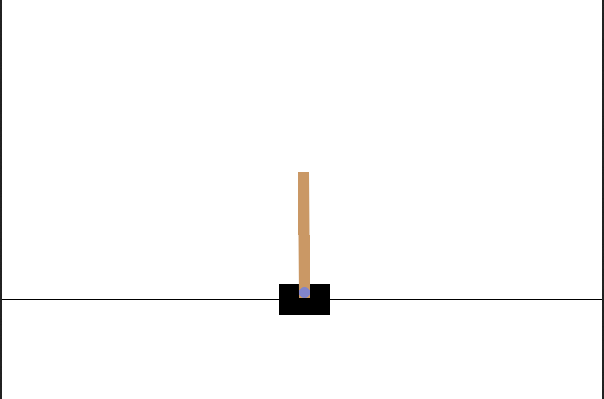
\includegraphics[width=0.6\textwidth]{./images/cartpole.png}
    
    \caption{Вид среды CartPole.}
    \label{fig:cartpole_scheme}
\end{figure}

\subsubsection{Пространство состояний}

Сенсорный аппарат агента крайне ограничен. В каждый момент времени t среда передает агенту вектор $S_t$, состоящий ровно из 4 непрерывных кинематических значений:

\begin{itemize}

  \item Позиция каретки: Текущее положение тележки на треке (от $-4.8$ до $4.8$ условных единиц). Такие значения обусловлены тем, что в оригинальном физическом эксперименте длина направляющего трека, по которому ездит тележка, составляла ровно 4.8 метра. Поскольку начальная позиция тележки находится ровно посередине трека, физический предел движения влево и вправо составляет ровно $\pm2.4$ метра. Этот предел был увеличен в два раза для того, чтобы среда успела зафиксировать окончательные значения при выходе агента за границы среды.
  \item Скорость каретки: Линейная скорость перемещения тележки.
  \item Угол отклонения шеста: Текущий угол наклона маятника относительно идеальной вертикали (в радианах).
  \item Угловая скорость шеста: Скорость падения или выравнивания маятника.

\end{itemize}

Именно этот вектор подается на входные узлы нейронной сети в процессе оценки приспособленности.

\subsubsection{Пространство действий}

Пространство возможных решений агента дискретно. На каждом шаге агент обязан выдать одну из двух команд:

\begin{itemize}
  
  \item 0: приложить фиксированный импульс силы, толкнув каретку влево.  
  \item 1: приложить фиксированный импульс силы, толкнув каретку вправо.

\end{itemize}

Важной особенностью является отсутствие действия «ничего не делать». Агент вынужден постоянно совершать микрокорректировки, что требует от нейросети быстрой реакции и точного балансирования между противоположными командами.

\subsubsection{Функция награды и условия завершения}

Награда в этой среде максимально проста: агент получает +1 за каждый такт времени, в течение которого шест остается в допустимом вертикальном положении.

Эпизод симуляции считается завершенным при выполнении любого из следующих условий:

\begin{enumerate}

  \item Падение: Угол отклонения шеста $\theta$ превысил допустимый порог (как правило, $\pm12^{\circ}$ или $\approx0.2095$ радиан от вертикали). Это ограничение основано на линейном приближении синуса малых углов.
  \item Выход за границы: Каретка уехала слишком далеко от центра экрана (позиция $x < -2.4$ или $x > 2.4$).
  \item Успех: Достигнут лимит времени симуляции (в версии среды CartPole-v1 этот лимит составляет 500 шагов).

\end{enumerate}

Агент должен достичь значения функции приспособленности в 500. Это означает, что нейросеть агента сформировала устойчивую стратегию балансировки, способную в рамках лимита среды поддерживать равновесие.

\subsubsection{Конфигурация алгоритма NEAT для среды CartPole}

Ниже приведены ключевые параметры, которые мы использовали в экспериментах:

\paragraph{Начальная топология и архитектура}

В соответствии с принципом постепенного усложнения структуры мы инициировали топологию нейросети с минимально возможной. Сеть не содержала скрытых слоев (num\_hidden = 0). Входной слой состоял из 4 нейронов, принимающих вектор состояния среды: позицию каретки, ее линейную скорость, угол отклонения шеста от вертикали и его угловую скорость. Выходной слой включал 2 нейрона, аппроксимирующих уверенность агента в необходимости приложения силы влево или вправо.

На старте эволюции мы применили также полную связность прямого распространения (initial\_connection = full\_direct). Выбор итогового дискретного действия агента осуществлялся путем вычисления максимума аргумента по вектору выходных значений сети. В качестве базовой функции активации для узлов применялась функция ReLU (activation\_default = relu).


\paragraph{Параметрические и структурные мутации:}

В процессе настройки \href{https://github.com/Isn0v/neat-training/blob/master/environments/cartpole/neat/neat.cfg}{конфигурационного файла}\footnote{\url{https://github.com/Isn0v/neat-training/blob/master/environments/cartpole/neat/neat.cfg}} мы намеренно сместили фокус на активную параметрическую адаптацию. На практике это работало так: алгоритм с высокой вероятностью (80\%, параметр weight\_mutate\_rate = 0.8) корректировал веса уже существующих связей, однако сама амплитуда этих изменений жестко сдерживалась параметром weight\_mutate\_power = 0.5.

Что касается структурного роста сети, мы решили отдать приоритет уплотнению связей, а не генерации новых узлов. Логика здесь проста: алгоритм должен по максимуму выработать потенциал текущей размерности графа, прежде чем наращивать его вычислительную сложность. Именно поэтому шанс образования нового синапса составил 50\% (conn\_add\_prob = 0.5), тогда как внедрение дополнительного скрытого нейрона допускалось значительно реже — лишь с вероятностью 20\% (node\_add\_prob = 0.2).

\paragraph{Параметры популяции и критерии сходимости:}

Размер эволюционирующей популяции мы задали на уровне 50 особей в каждом поколении (pop\_size = 50). Оценка приспособленности заключалась в суммарной награде, получаемой агентом за удержание маятника без падения и выхода за границы допустимой зоны.

В качестве критерия раннего останова и успешного завершения обучения мы установили порог приспособленности fitness\_threshold = 500, что соответствует максимально возможной оценке в стандартной спецификации среды CartPole-v1. Максимальный горизонт эволюции был ограничен 50 поколениями, однако, как показали дальнейшие эксперименты, алгоритм успешно находил оптимальную топологию задолго до исчерпания этого лимита.


\subsubsection{Архитектура и гиперпараметры агента DQN для среды CartPole}

Программная реализация алгоритма Deep Q-Network выполнялась с использованием библиотеки глубокого обучения PyTorch.

\paragraph{Архитектура нейронной сети:}

Чтобы аппроксимировать функцию ценности действий, мы спроектировали максимально компактную полносвязную сеть прямого распространения. На вход подается вектор из четырех элементов, описывающий текущую кинематику системы: координаты и скорости каретки, а также самого шеста. 

Скрытый слой мы намеренно ограничили всего 16 нейронами с функцией активации ReLU, потому что пространство состояний в среде CartPole-v1 довольно простое, и небольшая размерность сети не только спасает модель от переобучения, но и ощутимо ускоряет вычислительные проходы прямого и обратного распространения ошибки. На выходе формируются сигналы от двух нейронов с линейной активацией — они выдают предсказанные Q-значения для каждого из доступных действий (толчок влево или вправо). Итоговое решение агент принимает, просто выбирая аргумент максимального значения из этого вектора. 


\paragraph{Стратегия исследования и дисконтирование:}

Для соблюдения баланса между исследованием среды и эксплуатацией уже проверенных стратегий мы опирались на классическую $\epsilon$-жадную политику. На старте параметр исследования был выставлен в максимальное значение, равное 1. По мере обучения доля случайных действий плавно срезалась: на каждом шаге применялся коэффициент затухания $\epsilon_{decay} = 0.995$, пока исследование не упиралось в минимальный порог $\epsilon_{min} = 0.01$. Дополнительно мы задали высокий фактор дисконтирования ($\gamma = 0.99$). Он обеспечивал алгоритму необходимую «дальновидность», заставляя придавать огромный вес будущим потенциальным наградам, что является критическим условием для долгосрочной балансировки маятника.


\paragraph{Буфер памяти и процесс оптимизации:}

Для стабилизации процесса обучения нейронной сети использовался механизм воспроизведения опыта. Взаимодействия агента со средой сохранялись в циклический буфер памяти емкостью 10 000 переходов. На каждом шаге обучения (после накопления достаточного объема данных) из буфера случайным образом сэмплировался мини-батч размером 64 перехода. Это позволило разорвать временную корреляцию между последовательными состояниями и свести к минимуму дисперсию градиентов при обновлении весов.

Обновление весовых коэффициентов сети осуществлялось с помощью оптимизатора Adam со скоростью обучения 0.001. В качестве целевой метрики использовалась среднеквадратичная ошибка. Минимизируемая функция потерь $L$ строилась на основе отклонения текущего предсказания сети от целевого значения, вычисляемого согласно уравнению Беллмана:

\begin{equation}
  \label{eq:dqn_loss}
  L = \frac{1}{N} \sum_{t=0}^{T} ((r_t + \gamma \underset{a'}{max} Q(s_{t}, a')) - Q(s_t, a_t))^2
\end{equation}

где $N$ -- размер батча, $s_t$ и $a_t$ -- текущие состояние и действие, $r_t$ -- полученная награда, $s'_t$ -- следующее состояние, а $\gamma$ -- коэффициент дисконтирования.

Критерием успешного решения среды служило достижение суммарной награды в 500 баллов за один эпизод, что означает непрерывное удержание шеста в течение 500 тактов симуляции. По достижении этого порога веса модели (state\_dict) автоматически сохранялись для последующей демонстрации и анализа.